% !TeX program = lualatex
% ================================================================
% Polish Parallel Text Version of IntroducingPercentagesStarters
%
% Generated by the server using the following settings:
%
%   language            Polish (pol)
%   text direction      left to right
%   font                Noto Serif
%   fallback font       Noto Serif
%   built from          latex/starters/targeted/KS3/percentages/introducingPercentagesStarters.tex
%   vocabulary key      latex/starters/targeted/KS3/percentages/introducingPercentagesStarters/L2/pol/introducingPercentagesStarters_polishKey.tex
%   tier 3 vocabulary   green   RGB 0 128 0
%   English text        black   RGB 0 0 0
%   Polish text         purple  RGB 112 48 160
%   layout macros       version 3
%   sheet layout        version 1
%
% Please don't edit any information in this comment block - the server
% compares it against the current settings and rebuilds this file when
% they differ, so changes here would be overwritten. However, feel free
% to make updates to the LaTeX below if you want to edit it.
% ================================================================

\documentclass{beamer}
% ================================================================
% Copied from the English sheet this was translated from, so that
% anything it sets up for itself still works here
% ================================================================
\usepackage{tikz}
\usetikzlibrary{calc}
\usepackage{multicol}
\usepackage{amsmath}

% ================================================================
% Answer-overlay helpers
% ================================================================
\newcommand{\ablank}[1]{%
  \alt<2>{\textcolor{red}{#1}}{\underline{\phantom{#1}}}%
}
\newcommand{\ashow}[1]{\uncover<2->{\textcolor{red}{\small #1}}}
\newcommand{\ashowq}[1]{\alt<2->{\textcolor{red}{\small #1}}{?}}

% Answers drawn straight on to a TikZ diagram, revealed on overlay 2 like \ashow.
% Space is reserved on overlay 1, so the diagram does not move between slides.
\usetikzlibrary{overlay-beamer-styles}
\tikzset{
  ans/.style     = {red, thick, visible on=<2->},
  ansfill/.style = {red!15, visible on=<2->},
  anslab/.style  = {red, font=\tiny, visible on=<2->},
}

\title{Percentages: Starters}
\author{}
\date{}

% Characters this language's font has not got are borrowed from another,
% rather than being silently dropped - see docs/translated-sheet-latex.md
\directlua{%
  if luaotfload and luaotfload.add_fallback then
    luaotfload.add_fallback("eallatinfallback",
      { "Noto Serif:mode=harf;" })
  else
    tex.error("this luaotfload is too old to register a fallback font")
  end
}
\usepackage[english]{babel}
\babelprovide[import]{polish}
\babelfont[polish]{rm}[Renderer=Harfbuzz, BoldFont={Noto Serif}, ItalicFont={Noto Serif}, BoldItalicFont={Noto Serif}, RawFeature={fallback=eallatinfallback}]{Noto Serif}
\babelfont[polish]{sf}[Renderer=Harfbuzz, BoldFont={Noto Serif}, ItalicFont={Noto Serif}, BoldItalicFont={Noto Serif}, RawFeature={fallback=eallatinfallback}]{Noto Serif}
\newcommand{\ealtext}[1]{\foreignlanguage{polish}{#1}}
\newcommand{\ealtextblock}[1]{{\raggedright\foreignlanguage{polish}{#1}\par}}
% ================================================================
% EAL layout helpers
% ================================================================
\usepackage{xcolor}

\definecolor{ealkeycolour}{RGB}{0,128,0}
\definecolor{ealenglish}{RGB}{0,0,0}
\definecolor{ealtwocolour}{RGB}{112,48,160}

\newsavebox{\ealboxen}
\newsavebox{\ealboxtr}
\newlength{\ealglosswd}
\newlength{\ealglossraise}
\setlength{\ealglossraise}{1.15em}

% a tier 3 word, in English and in translation alike
\newcommand{\ealkey}[1]{\textcolor{ealkeycolour}{#1}}
\newcommand{\ealkeytr}[1]{\textcolor{ealkeycolour}{\ealtext{#1}}}

% One translated word above one English word. Built from kernel
% primitives, never a tabular, which would break wherever the sheet
% loads array, booktabs or tabularx. The box is as wide as the wider of
% the two, so a long translation pushes its neighbours aside instead of
% overlapping them, and it claims its full height so a table row or a
% TikZ node makes room for it.
\newcommand{\ealgloss}[2]{%
  \sbox{\ealboxen}{\ealkey{#1}}%
  \sbox{\ealboxtr}{\small\textcolor{ealtwocolour}{\ealtext{#2}}}%
  \setlength{\ealglosswd}{\wd\ealboxen}%
  \ifdim\wd\ealboxtr>\ealglosswd\setlength{\ealglosswd}{\wd\ealboxtr}\fi
  \leavevmode
  \makebox[\ealglosswd][c]{%
    \makebox[0pt][c]{\usebox{\ealboxen}}%
    \makebox[0pt][c]{\raisebox{\ealglossraise}{\usebox{\ealboxtr}}}%
  }%
}

% opens up line spacing around a block of glosses, so the raised
% translations sit clear of the line above
\newenvironment{ealglossed}{\par\linespread{2.1}\selectfont\ignorespaces}{\par}

% a whole translated sentence above its English counterpart. block level,
% so it does not belong inside a tabular cell
\newcommand{\ealpara}[2]{%
  \par\addvspace{0.5\baselineskip}%
  {\color{ealtwocolour}\ealtextblock{#1}}%
  \penalty200
  {\color{ealenglish}#2\par}%
  \addvspace{0.5\baselineskip}%
}

\begin{document}

\frame{\titlepage}

%------------------------------------------------------------------
% SLIDE 1 (1 of 3): What is a Percentage?
%------------------------------------------------------------------
\begin{frame}[t]{Starter (1 of 3)}
\begin{columns}
\column{0.4\textwidth}
\begin{center}
\vspace{-1.5em}
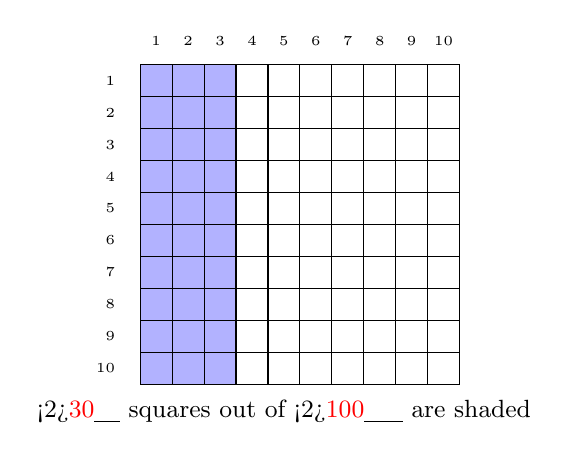
\begin{tikzpicture}[scale=0.78]
% 10×10 grid; first 3 columns shaded = 30 squares
\foreach \col in {0,...,9}{
  \foreach \row in {0,...,9}{
    \ifnum\col<3
      \fill[blue!30] (\col*0.52,\row*0.52) rectangle ++(0.52,0.52);
    \fi
    \draw (\col*0.52,\row*0.52) rectangle ++(0.52,0.52);
  }
}
% Column numbers 1--10 along the top
\foreach \col in {0,...,9}{
  \node[font=\tiny, above] at (\col*0.52+0.26, 5.2+0.15) {\number\numexpr\col+1};
}
% Row numbers 1--10 along the left side (bottom = 1, top = 10)
\foreach \row in {0,...,9}{
  \node[font=\tiny, left] at (-0.25, \row*0.52+0.26) {\number\numexpr10-\row};
}
\node at (2.34,-0.45) {\small \ablank{30} squares out of \ablank{100} are shaded };
\end{tikzpicture}
\end{center}

\column{0.6\textwidth}
\vspace{-1.5em}
\begin{enumerate}
  \item \ealpara{Na diagramie ile kwadratów jest zacienionych? \ablank{30}}{In the diagram how many squares are shaded? \ablank{30}}
  \item \ealpara{Ile jest wszystkich kwadratów? \ablank{100}}{How many total squares are there? \ablank{100}}
  \item \ealpara{$70 + 30 = \ablank{100}$}{$70 + 30 = \ablank{100}$}
  \item \ealpara{$25 \times 4 = \ablank{100}$}{$25 \times 4 = \ablank{100}$}
\end{enumerate}
\end{columns}
\end{frame}

%------------------------------------------------------------------
% SLIDE 1 (2 of 3): What is a Percentage?
%------------------------------------------------------------------
\begin{frame}[t]{Starter (2 of 3)}
\begin{columns}
\column{0.4\textwidth}
\begin{center}
\vspace{-1.5em}
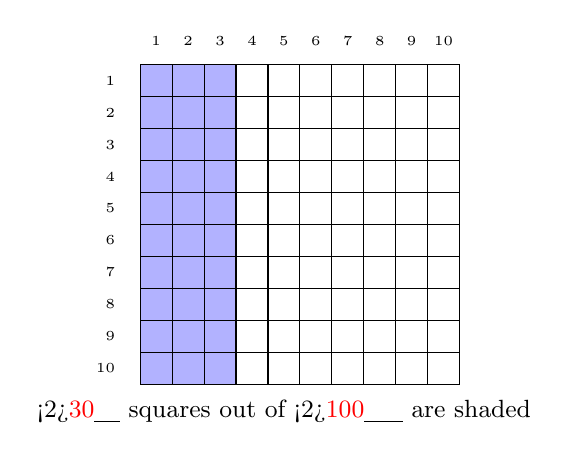
\begin{tikzpicture}[scale=0.78]
\foreach \col in {0,...,9}{
  \foreach \row in {0,...,9}{
    \ifnum\col<3
      \fill[blue!30] (\col*0.52,\row*0.52) rectangle ++(0.52,0.52);
    \fi
    \draw (\col*0.52,\row*0.52) rectangle ++(0.52,0.52);
  }
}
\foreach \col in {0,...,9}{
  \node[font=\tiny, above] at (\col*0.52+0.26, 5.2+0.15) {\number\numexpr\col+1};
}
\foreach \row in {0,...,9}{
  \node[font=\tiny, left] at (-0.25, \row*0.52+0.26) {\number\numexpr10-\row};
}
\node at (2.34,-0.45) {\small \ablank{30} squares out of \ablank{100} are shaded };
\end{tikzpicture}
\end{center}

\column{0.6\textwidth}
\vspace{-1.5em}
\begin{enumerate}
\setcounter{enumi}{4}
  \item \ealpara{Jaki \ealkeytr{ułamek} kwadratu jest zacieniony: \ashow{$\tfrac{30}{100}$}}{What \ealkey{fraction} of the square is shaded: \ashow{$\tfrac{30}{100}$}}
  \item \ealpara{``\ealkeytr{Procent}'' oznacza ``na \ablank{100}''.}{``\ealkey{Per cent}'' means ``out of \ablank{100}''.}
  \item \ealpara{Zacieniony \ealkeytr{ułamek} $= \ablank{30\%}$}{The shaded \ealkey{fraction} $= \ablank{30\%}$}
\end{enumerate}
\end{columns}
\end{frame}

%------------------------------------------------------------------
% SLIDE 1 (3 of 3): What is a Percentage?
%------------------------------------------------------------------
\begin{frame}[t]{Starter (3 of 3)}
\begin{enumerate}
\setcounter{enumi}{7}
  \item \ealpara{Zapisz $\dfrac{1}{2}$ jako \ealkeytr{procent}. \ablank{$50\%$}}{Write $\dfrac{1}{2}$ as a \ealkey{percentage}. \ablank{$50\%$}}
  \item \ealpara{Zapisz $\dfrac{1}{4}$ jako \ealkeytr{procent}. \ablank{$25\%$}}{Write $\dfrac{1}{4}$ as a \ealkey{percentage}. \ablank{$25\%$}}
  \item \ealpara{Zapisz $\dfrac{5}{4}$ jako \ealkeytr{procent}. \ablank{$125\%$}}{Write $\dfrac{5}{4}$ as a \ealkey{percentage}. \ablank{$125\%$}}
\end{enumerate}
\end{frame}

%------------------------------------------------------------------
% SLIDE 2 (1 of 3): Fractions → Percentages
%------------------------------------------------------------------
\begin{frame}[t]{Starter (1 of 3)}
\begin{columns}
\column{0.48\textwidth}
\vspace{-4em}
\begin{center}
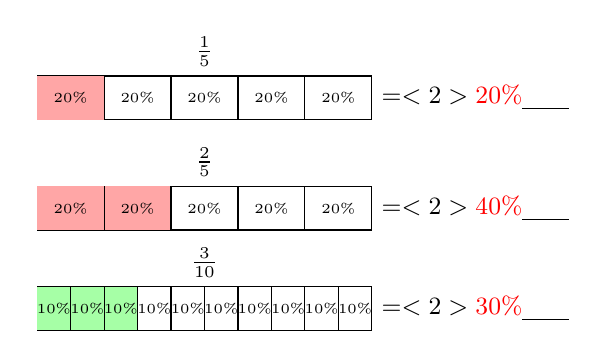
\begin{tikzpicture}[scale=0.85]
% bar 1/5
\draw (0,0) rectangle (5.0,0.65);
\fill[red!35] (0,0) rectangle (1.0,0.65);
\foreach \x in {1,2,3,4} \draw (\x,0) -- (\x,0.65);
\foreach \i in {0,1,2,3,4}
  \node[font=\tiny] at (\i +0.50,0.325) {20\%};
\node[above,font=\small] at (2.5,0.65) {$\tfrac{1}{5}$};
\node[right,font=\small] at (5.0,0.325) {$=\ablank{20\%}$};

% bar 2/5
\draw (0,-1.65) rectangle (5.0,-1.0);
\fill[red!35] (0,-1.65) rectangle (2.0,-1.0);
\foreach \x in {1,2,3,4} \draw (\x,-1.65) -- (\x,-1.0);
\foreach \i in {0,1,2,3,4}
  \node[font=\tiny] at (\i+0.50,-1.325) {20\%};
\node[above,font=\small] at (2.5,-1.0) {$\tfrac{2}{5}$};
\node[right,font=\small] at (5.0,-1.325) {$=\ablank{40\%}$};

% bar 3/10
\draw (0,-3.15) rectangle (5.0,-2.5);
\fill[green!35] (0,-3.15) rectangle (1.50,-2.5);
\foreach \x in {0.50,1.0,...,5.00} \draw (\x,-3.15) -- (\x,-2.5);
\foreach \i in {0,...,9}
  \node[font=\tiny] at (\i*0.50+0.25,-2.825) {10\%};
\node[above,font=\small] at (2.5,-2.5) {$\tfrac{3}{10}$};
\node[right,font=\small] at (5.0,-2.825) {$=\ablank{30\%}$};
\end{tikzpicture}
\end{center}

\column{0.52\textwidth}
\vspace{-2em}
\begin{enumerate}
  \item \ealpara{$3 \times 20 = \ablank{60}$}{$3 \times 20 = \ablank{60}$}
  \item \ealpara{$7 \times 10 = \ablank{70}$}{$7 \times 10 = \ablank{70}$}
  \item \ealpara{$\dfrac{1}{5} = \ablank{20\%}$}{$\dfrac{1}{5} = \ablank{20\%}$}
  \item \ealpara{$\dfrac{2}{5} = \ablank{40\%}$}{$\dfrac{2}{5} = \ablank{40\%}$}
\end{enumerate}
\end{columns}
\end{frame}

%------------------------------------------------------------------
% SLIDE 2 (2 of 3): Fractions → Percentages
%------------------------------------------------------------------
\begin{frame}[t]{Starter (2 of 3)}
\begin{columns}
\column{0.48\textwidth}
\vspace{-4em}
\begin{center}
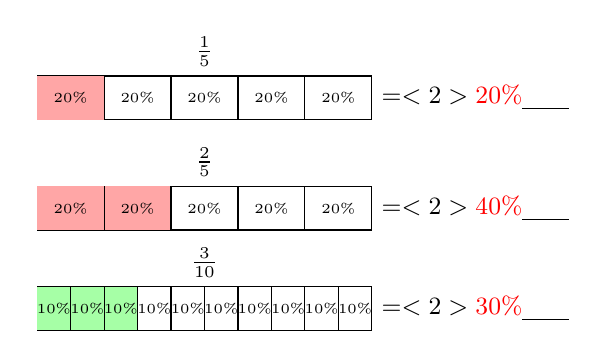
\begin{tikzpicture}[scale=0.85]
\draw (0,0) rectangle (5.0,0.65);
\fill[red!35] (0,0) rectangle (1.0,0.65);
\foreach \x in {1,2,3,4} \draw (\x,0) -- (\x,0.65);
\foreach \i in {0,1,2,3,4}
  \node[font=\tiny] at (\i +0.50,0.325) {20\%};
\node[above,font=\small] at (2.5,0.65) {$\tfrac{1}{5}$};
\node[right,font=\small] at (5.0,0.325) {$=\ablank{20\%}$};

\draw (0,-1.65) rectangle (5.0,-1.0);
\fill[red!35] (0,-1.65) rectangle (2.0,-1.0);
\foreach \x in {1,2,3,4} \draw (\x,-1.65) -- (\x,-1.0);
\foreach \i in {0,1,2,3,4}
  \node[font=\tiny] at (\i+0.50,-1.325) {20\%};
\node[above,font=\small] at (2.5,-1.0) {$\tfrac{2}{5}$};
\node[right,font=\small] at (5.0,-1.325) {$=\ablank{40\%}$};

\draw (0,-3.15) rectangle (5.0,-2.5);
\fill[green!35] (0,-3.15) rectangle (1.50,-2.5);
\foreach \x in {0.50,1.0,...,5.00} \draw (\x,-3.15) -- (\x,-2.5);
\foreach \i in {0,...,9}
  \node[font=\tiny] at (\i*0.50+0.25,-2.825) {10\%};
\node[above,font=\small] at (2.5,-2.5) {$\tfrac{3}{10}$};
\node[right,font=\small] at (5.0,-2.825) {$=\ablank{30\%}$};
\end{tikzpicture}
\end{center}

\column{0.52\textwidth}
\vspace{-2em}
\begin{enumerate}
\setcounter{enumi}{4}
  \item \ealpara{$\dfrac{3}{10} = \ablank{30\%}$}{$\dfrac{3}{10} = \ablank{30\%}$}
  \item \ealpara{$\dfrac{\text{\ashowq{7}}}{10} = 70\%$}{$\dfrac{\text{\ashowq{7}}}{10} = 70\%$}
  \item \ealpara{$\dfrac{1}{\text{\ashowq{4}}} = 25\%$}{$\dfrac{1}{\text{\ashowq{4}}} = 25\%$}
  \item \ealpara{$\dfrac{2}{25} = \ablank{8\%}$}{$\dfrac{2}{25} = \ablank{8\%}$}
\end{enumerate}
\end{columns}
\end{frame}

%------------------------------------------------------------------
% SLIDE 2 (3 of 3): Fractions → Percentages
%------------------------------------------------------------------
\begin{frame}[t]{Starter (3 of 3)}
\begin{enumerate}
\setcounter{enumi}{8}
  \item \ealpara{$\dfrac{7}{8} = \ablank{87.5\%}$}{$\dfrac{7}{8} = \ablank{87.5\%}$}
  \item \ealpara{$\dfrac{5}{3}={}$\ablank{$166.\dot{6}\%$}}{$\dfrac{5}{3}={}$\ablank{$166.\dot{6}\%$}}
  \item \ealpara{Uzupełnij \ealkeytr{zamianę}: \\[2pt] $\dfrac{\text{\ashowq{3}}}{4} = \dfrac{75}{\text{\ashowq{100}}} = 75\%$}{Complete the \ealkey{conversion}: \\[2pt] $\dfrac{\text{\ashowq{3}}}{4} = \dfrac{75}{\text{\ashowq{100}}} = 75\%$}
\end{enumerate}
\end{frame}

%------------------------------------------------------------------
% SLIDE 3 (1 of 3): Converting Fractions to Percentages
%------------------------------------------------------------------
\begin{frame}[t]{Starter (1 of 3)}
\ealpara{Pytania}{\textbf{Questions}}
\begin{enumerate}
  \item \ealpara{Zapisz $\frac{1}{2}$ jako \ealkeytr{procent}. \ablank{$50\%$}}{Write $\frac{1}{2}$ as a \ealkey{percentage}. \ablank{$50\%$}}
  \item \ealpara{Zapisz $\frac{3}{10}$ jako \ealkeytr{procent}. \ablank{$30\%$}}{Write $\frac{3}{10}$ as a \ealkey{percentage}. \ablank{$30\%$}}
  \item \ealpara{Co oznacza “\ealkeytr{procent}”? \ablank{na 100}}{What does “\ealkey{per cent}” mean? \ablank{out of 100}}
\end{enumerate}
\end{frame}

%------------------------------------------------------------------
% SLIDE 3 (2 of 3): Converting Fractions to Percentages
%------------------------------------------------------------------
\begin{frame}[t]{Starter (2 of 3)}
\begin{columns}
\column{0.35\textwidth}
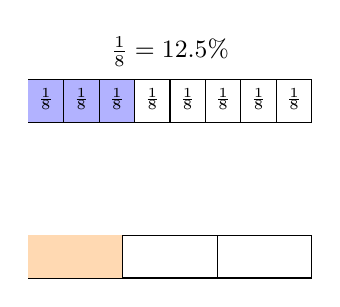
\begin{tikzpicture}[scale=0.9]
\draw (0,0) rectangle (4,0.6);
\fill[blue!30] (0,0) rectangle (1.5,0.6);
\foreach \x in {0.5,1.0,1.5,2.0,2.5,3.0,3.5}
  \draw (\x,0) -- (\x,0.6);
\foreach \i in {0.5,1.0,1.5,2.0,2.5,3.0,3.5,4.0}
  \node[font=\tiny] at (\i-0.25,0.325) {$\frac{1}{8}$};
\node[above,font=\small] at (2,0.65) {$\frac{1}{8} = 12.5\%$};
\draw (0,-2.2) rectangle (4,-1.6);
\fill[orange!30] (0,-2.2) rectangle (1.333,-1.6);
\draw (1.333,-2.2) -- (1.333,-1.6);
\draw (2.667,-2.2) -- (2.667,-1.6);
\end{tikzpicture}

\column{0.65\textwidth}
\ealpara{Pytania}{\textbf{Questions}}
\begin{enumerate}
\setcounter{enumi}{3}
  \item \ealpara{\ealkeytr{Zamień} $\frac{3}{8}$ na \ealkeytr{procent}. \ablank{$37.5\%$}}{\ealkey{Convert} $\frac{3}{8}$ to a \ealkey{percentage}. \ablank{$37.5\%$}}
  \item \ealpara{Jaki \ealkeytr{procent} drugiego paska jest zacieniony na pomarańczowo? \ablank{$33.\dot{3}\%$}}{What \ealkey{percentage} of the second bar is shaded orange? \ablank{$33.\dot{3}\%$}}
  \item \ealpara{\ealkeytr{Zamień} $\frac{2}{3}$ na \ealkeytr{procent}. \ablank{$66.\dot{6}\%$}}{\ealkey{Convert} $\frac{2}{3}$ to a \ealkey{percentage}. \ablank{$66.\dot{6}\%$}}
\end{enumerate}
\end{columns}
\end{frame}

%------------------------------------------------------------------
% SLIDE 3 (3 of 3): Converting Fractions to Percentages
%------------------------------------------------------------------
\begin{frame}[t]{Starter (3 of 3)}
\ealpara{Pytania}{\textbf{Questions}}
\begin{enumerate}
\setcounter{enumi}{6}
  \item \ealpara{Jaki jest $\frac{4}{3}$ jako \ealkeytr{procent}, \ealkeytr{zaokrąglij} swój \ealkeytr{procent} do jednego \ealkeytr{miejsca dziesiętnego}. \ablank{$133.3\%$}}{What is $\frac{4}{3}$ as a \ealkey{percentage}, \ealkey{round} your \ealkey{percentage} to one \ealkey{decimal place}. \ablank{$133.3\%$}}
  \item \ealpara{Jakiemu \ealkeytr{ułamkowi} równa się $0.1\%$? \ashow{$\frac{1}{1000}$}}{What \ealkey{fraction} does $0.1\%$ equal? \ashow{$\frac{1}{1000}$}}
  \item \ealpara{Jakiemu \ealkeytr{ułamkowi} równa się $0.003\%$? \ashow{$\frac{3}{100,000}$}}{What \ealkey{fraction} does $0.003\%$ equal? \ashow{$\frac{3}{100,000}$}}
\end{enumerate}
\end{frame}

%------------------------------------------------------------------
% SLIDE 4 (1 of 3): Adding Fractions and Percentages
%------------------------------------------------------------------
\begin{frame}[t]{Starter (1 of 3)}
\begin{columns}
\column{0.35\textwidth}
\begin{center}
\vspace{-5em}
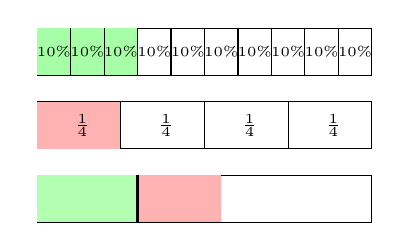
\begin{tikzpicture}[scale=0.85]
\draw (0,0) rectangle (5.0,0.7);
\fill[green!35] (0,0) rectangle (1.50,0.7);
\foreach \x in {0.50,1.0,...,5.00} \draw (\x,0) -- (\x,0.7);
\foreach \i in {0,...,9}
  \node[font=\tiny] at (\i*0.50+0.25,0.35) {10\%};

\draw (0,-1.1) rectangle (5,-0.4);
\fill[red!30] (0,-1.1) rectangle (1.25,-0.4);
\foreach \x in {1.25,2.5,3.75} \draw (\x,-1.1) -- (\x,-0.4);
\foreach \i in {0,...,3}
    \node[font=\tiny] at (\i*1.25+0.675,-0.75) {$\frac{1}{4}$};
    
\draw (0,-2.2) rectangle (5,-1.5);
\fill[green!30] (0,-2.2) rectangle (1.5,-1.5);
\fill[red!30] (1.5,-2.2) rectangle (2.75,-1.5);
\draw[thick] (1.5,-2.2) -- (1.5,-1.5);
\end{tikzpicture}
\end{center}

\column{0.7\textwidth}
\vspace{-2em}
\begin{enumerate}
  \item \ealpara{$50\% + 50\% = \ablank{100\%}$}{$50\% + 50\% = \ablank{100\%}$}
  \item \ealpara{$25\% + 25\% = \ablank{50\%}$}{$25\% + 25\% = \ablank{50\%}$}
  \item \ealpara{Zapisz $\frac{1}{5}$ jako \ealkeytr{procent}: \ablank{$20\%$}}{Write $\frac{1}{5}$ as a \ealkey{percentage}: \ablank{$20\%$}}
  \item \ealpara{Uzupełnij \ealkeytr{sumę} przedstawioną na diagramie: \\[0.2em] $ 3 \times \text{\ashowq{10}}\% + \frac{1}{\text{\ashowq{4}}} = 30\% + 25\% = 55\% $}{Complete the \ealkey{sum} represented by the diagram: \\[0.2em] $ 3 \times \text{\ashowq{10}}\% + \frac{1}{\text{\ashowq{4}}} = 30\% + 25\% = 55\% $}
\end{enumerate}
\end{columns}
\end{frame}

%------------------------------------------------------------------
% SLIDE 4 (2 of 3): Adding Fractions and Percentages
%------------------------------------------------------------------
\begin{frame}[t]{Starter (2 of 3)}
\begin{enumerate}
\setcounter{enumi}{4}
  \item \ealpara{$20\%+\dfrac{3}{10}=\ablank{50\%}$}{$20\%+\dfrac{3}{10}=\ablank{50\%}$}
  \item \ealpara{$\dfrac{1}{2}+15\%=\ablank{65\%}$}{$\dfrac{1}{2}+15\%=\ablank{65\%}$}
  \item \ealpara{$45\%+\dfrac{1}{5}=\ablank{65\%}$}{$45\%+\dfrac{1}{5}=\ablank{65\%}$}
\end{enumerate}
\end{frame}

%------------------------------------------------------------------
% SLIDE 4 (3 of 3): Adding Fractions and Percentages
%------------------------------------------------------------------
\begin{frame}[t]{Starter (3 of 3)}
\begin{enumerate}
\setcounter{enumi}{7}
  \item \ealpara{Co jest większe: $\dfrac{3}{8}$ czy $40\%$? \ablank{$40\%$ ($\tfrac{3}{8}=37.5\%$)}}{Which is larger: $\dfrac{3}{8}$ or $40\%$? \ablank{$40\%$ ($\tfrac{3}{8}=37.5\%$)}}
  \item \ealpara{$\dfrac{2}{5}+\dfrac{3}{10}+20\%=\ablank{90\%}$}{$\dfrac{2}{5}+\dfrac{3}{10}+20\%=\ablank{90\%}$}
  \item \ealpara{Klasa kończy $\tfrac{1}{3}$ projektu, a potem jeszcze $20\%$. Jaki \ealkeytr{procent} pracy ukończyli łącznie? \ashow{$33.\dot{3}\%+20\%=53.\dot{3}\%$}}{A class finishes $\tfrac{1}{3}$ of a project, then $20\%$ more. What \ealkey{percentage} have they completed in total? \ashow{$33.\dot{3}\%+20\%=53.\dot{3}\%$}}
\end{enumerate}
\end{frame}

%------------------------------------------------------------------
% SLIDE 7 (1 of 3): Decimals to Percentages
%------------------------------------------------------------------
\begin{frame}[t]{Starter (1 of 3)}
\begin{columns}
\column{0.4\textwidth}
\begin{center}
\vspace{-1em}
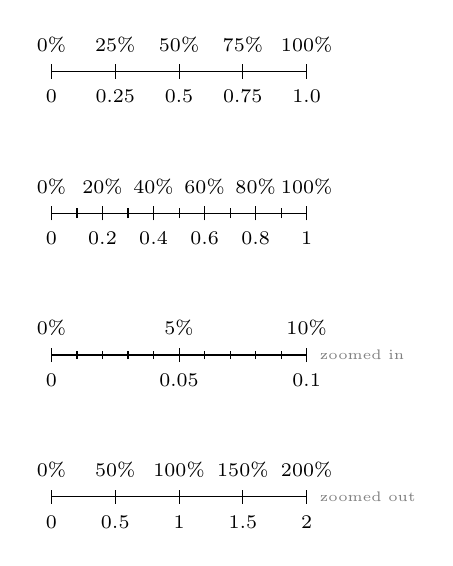
\begin{tikzpicture}[scale=0.9, every node/.style={font=\scriptsize}]
\def\Y{0}
\def\W{3.6}
\draw (0,\Y) -- (\W,\Y);
\foreach \frac/\dec/\pct in {%
    0/{0}/{0\%}, 1/{0.25}/{25\%}, 2/{0.5}/{50\%},
    3/{0.75}/{75\%}, 4/{1.0}/{100\%}}{
  \pgfmathsetmacro\xx{\frac*\W/4}
  \draw (\xx,\Y-0.10) -- (\xx,\Y+0.10);
  \node[below] at (\xx,\Y-0.13) {\dec};
  \node[above] at (\xx,\Y+0.13) {\pct};
}
\def\Y{-2.0}
\draw (0,\Y) -- (\W,\Y);
\foreach \k in {0,1,...,10}{
  \pgfmathsetmacro\xx{\k*\W/10}
  \pgfmathsetmacro\dec{\k/10}
  \ifodd\k
    \draw (\xx,\Y-0.07) -- (\xx,\Y+0.07);
  \else
    \draw (\xx,\Y-0.10) -- (\xx,\Y+0.10);
    \node[below] at (\xx,\Y-0.13) {\pgfmathprintnumber[fixed,precision=1]{\dec}};
    \pgfmathsetmacro\pct{int(\k*10)}
    \node[above] at (\xx,\Y+0.13) {\pct\%};
  \fi
}
\pgfmathsetmacro\ta{0.92*\W}
\def\Y{-4.0}
\draw (0,\Y) -- (\W,\Y);
\foreach \k/\dec/\pct in {0/{0}/{0\%}, 1/{0.05}/{5\%}, 2/{0.1}/{10\%}}{
  \pgfmathsetmacro\xx{\k*\W/2}
  \draw (\xx,\Y-0.10) -- (\xx,\Y+0.10);
  \node[below] at (\xx,\Y-0.13) {\dec};
  \node[above] at (\xx,\Y+0.13) {\pct};
}
\foreach \k in {1,2,...,9}{
  \pgfmathsetmacro\xx{\k*\W/10}
  \draw (\xx,\Y-0.06) -- (\xx,\Y+0.06);
}
\node[right,gray] at (\W+0.05,\Y) {\tiny zoomed in};
\def\Y{-6.0}
\draw (0,\Y) -- (\W,\Y);
\foreach \k in {0,1,2,3,4}{
  \pgfmathsetmacro\xx{\k*\W/4}
  \pgfmathsetmacro\dec{\k/2}
  \pgfmathsetmacro\pct{int(\k*50)}
  \draw (\xx,\Y-0.10) -- (\xx,\Y+0.10);
  \node[below] at (\xx,\Y-0.13) {\pgfmathprintnumber[fixed,precision=1]{\dec}};
  \node[above] at (\xx,\Y+0.13) {\pct\%};
}
\node[right,gray] at (\W+0.05,\Y) {\tiny zoomed out};
\end{tikzpicture}
\end{center}

\column{0.6\textwidth}
\begin{enumerate}
  \item \ealpara{$0.6 + 0.4 = \ablank{1}$}{$0.6 + 0.4 = \ablank{1}$}
  \item \ealpara{$0.25 \times 4 = \ablank{1}$}{$0.25 \times 4 = \ablank{1}$}
  \item \ealpara{Zapisz $\frac{3}{10}$ jako \ealkeytr{ułamek dziesiętny}: \ablank{$0.3$}}{Write $\frac{3}{10}$ as a \ealkey{decimal}: \ablank{$0.3$}}
  \item \ealpara{Zapisz $\frac{7}{100}$ jako \ealkeytr{ułamek dziesiętny}: \ablank{$0.07$}}{Write $\frac{7}{100}$ as a \ealkey{decimal}: \ablank{$0.07$}}
  \item \ealpara{$0.5   = \ablank{50\%}$}{$0.5   = \ablank{50\%}$}
\end{enumerate}
\end{columns}
\end{frame}

%------------------------------------------------------------------
% SLIDE 7 (2 of 3): Decimals to Percentages
%------------------------------------------------------------------
\begin{frame}[t]{Starter (2 of 3)}
\begin{columns}
\column{0.4\textwidth}
\begin{center}
\vspace{-1em}
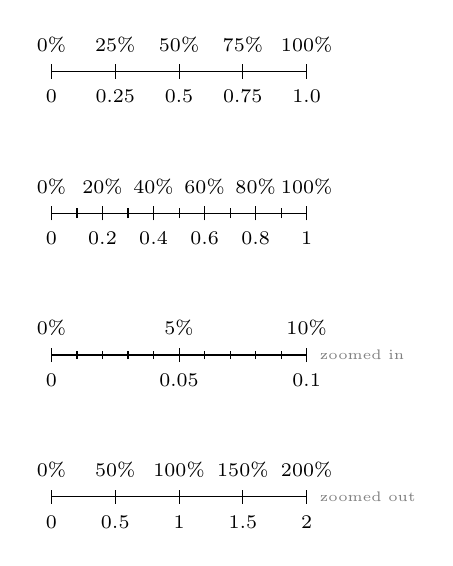
\begin{tikzpicture}[scale=0.9, every node/.style={font=\scriptsize}]
\def\Y{0}
\def\W{3.6}
\draw (0,\Y) -- (\W,\Y);
\foreach \frac/\dec/\pct in {%
    0/{0}/{0\%}, 1/{0.25}/{25\%}, 2/{0.5}/{50\%},
    3/{0.75}/{75\%}, 4/{1.0}/{100\%}}{
  \pgfmathsetmacro\xx{\frac*\W/4}
  \draw (\xx,\Y-0.10) -- (\xx,\Y+0.10);
  \node[below] at (\xx,\Y-0.13) {\dec};
  \node[above] at (\xx,\Y+0.13) {\pct};
}
\def\Y{-2.0}
\draw (0,\Y) -- (\W,\Y);
\foreach \k in {0,1,...,10}{
  \pgfmathsetmacro\xx{\k*\W/10}
  \pgfmathsetmacro\dec{\k/10}
  \ifodd\k
    \draw (\xx,\Y-0.07) -- (\xx,\Y+0.07);
  \else
    \draw (\xx,\Y-0.10) -- (\xx,\Y+0.10);
    \node[below] at (\xx,\Y-0.13) {\pgfmathprintnumber[fixed,precision=1]{\dec}};
    \pgfmathsetmacro\pct{int(\k*10)}
    \node[above] at (\xx,\Y+0.13) {\pct\%};
  \fi
}
\pgfmathsetmacro\ta{0.92*\W}
\def\Y{-4.0}
\draw (0,\Y) -- (\W,\Y);
\foreach \k/\dec/\pct in {0/{0}/{0\%}, 1/{0.05}/{5\%}, 2/{0.1}/{10\%}}{
  \pgfmathsetmacro\xx{\k*\W/2}
  \draw (\xx,\Y-0.10) -- (\xx,\Y+0.10);
  \node[below] at (\xx,\Y-0.13) {\dec};
  \node[above] at (\xx,\Y+0.13) {\pct};
}
\foreach \k in {1,2,...,9}{
  \pgfmathsetmacro\xx{\k*\W/10}
  \draw (\xx,\Y-0.06) -- (\xx,\Y+0.06);
}
\node[right,gray] at (\W+0.05,\Y) {\tiny zoomed in};
\def\Y{-6.0}
\draw (0,\Y) -- (\W,\Y);
\foreach \k in {0,1,2,3,4}{
  \pgfmathsetmacro\xx{\k*\W/4}
  \pgfmathsetmacro\dec{\k/2}
  \pgfmathsetmacro\pct{int(\k*50)}
  \draw (\xx,\Y-0.10) -- (\xx,\Y+0.10);
  \node[below] at (\xx,\Y-0.13) {\pgfmathprintnumber[fixed,precision=1]{\dec}};
  \node[above] at (\xx,\Y+0.13) {\pct\%};
}
\node[right,gray] at (\W+0.05,\Y) {\tiny zoomed out};
\end{tikzpicture}
\end{center}

\column{0.6\textwidth}
\begin{enumerate}
\setcounter{enumi}{5}
  \item \ealpara{$0.3   = \ablank{30\%}$}{$0.3   = \ablank{30\%}$}
  \item \ealpara{$0.75  = \ablank{75\%}$}{$0.75  = \ablank{75\%}$}
  \item \ealpara{$0.08  = \ablank{8\%}$}{$0.08  = \ablank{8\%}$}
  \item \ealpara{$0.125 = \ablank{12.5\%}$}{$0.125 = \ablank{12.5\%}$}
\end{enumerate}
\end{columns}
\end{frame}

%------------------------------------------------------------------
% SLIDE 7 (3 of 3): Decimals to Percentages
%------------------------------------------------------------------
\begin{frame}[t]{Starter (3 of 3)}
\begin{columns}
\column{0.4\textwidth}
\begin{center}
\vspace{-1em}
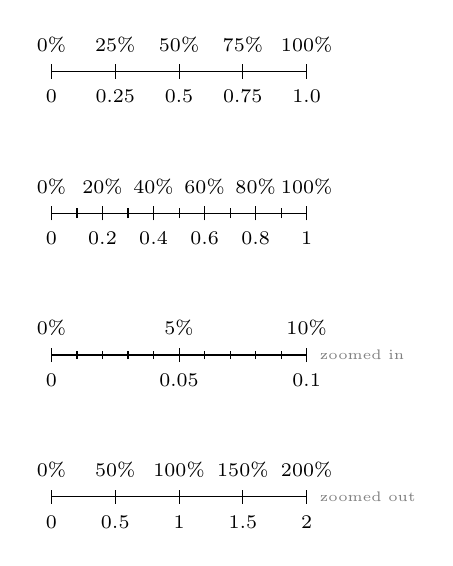
\begin{tikzpicture}[scale=0.9, every node/.style={font=\scriptsize}]
\def\Y{0}
\def\W{3.6}
\draw (0,\Y) -- (\W,\Y);
\foreach \frac/\dec/\pct in {%
    0/{0}/{0\%}, 1/{0.25}/{25\%}, 2/{0.5}/{50\%},
    3/{0.75}/{75\%}, 4/{1.0}/{100\%}}{
  \pgfmathsetmacro\xx{\frac*\W/4}
  \draw (\xx,\Y-0.10) -- (\xx,\Y+0.10);
  \node[below] at (\xx,\Y-0.13) {\dec};
  \node[above] at (\xx,\Y+0.13) {\pct};
}
\def\Y{-2.0}
\draw (0,\Y) -- (\W,\Y);
\foreach \k in {0,1,...,10}{
  \pgfmathsetmacro\xx{\k*\W/10}
  \pgfmathsetmacro\dec{\k/10}
  \ifodd\k
    \draw (\xx,\Y-0.07) -- (\xx,\Y+0.07);
  \else
    \draw (\xx,\Y-0.10) -- (\xx,\Y+0.10);
    \node[below] at (\xx,\Y-0.13) {\pgfmathprintnumber[fixed,precision=1]{\dec}};
    \pgfmathsetmacro\pct{int(\k*10)}
    \node[above] at (\xx,\Y+0.13) {\pct\%};
  \fi
}
\pgfmathsetmacro\ta{0.92*\W}
\def\Y{-4.0}
\draw (0,\Y) -- (\W,\Y);
\foreach \k/\dec/\pct in {0/{0}/{0\%}, 1/{0.05}/{5\%}, 2/{0.1}/{10\%}}{
  \pgfmathsetmacro\xx{\k*\W/2}
  \draw (\xx,\Y-0.10) -- (\xx,\Y+0.10);
  \node[below] at (\xx,\Y-0.13) {\dec};
  \node[above] at (\xx,\Y+0.13) {\pct};
}
\foreach \k in {1,2,...,9}{
  \pgfmathsetmacro\xx{\k*\W/10}
  \draw (\xx,\Y-0.06) -- (\xx,\Y+0.06);
}
\node[right,gray] at (\W+0.05,\Y) {\tiny zoomed in};
\def\Y{-6.0}
\draw (0,\Y) -- (\W,\Y);
\foreach \k in {0,1,2,3,4}{
  \pgfmathsetmacro\xx{\k*\W/4}
  \pgfmathsetmacro\dec{\k/2}
  \pgfmathsetmacro\pct{int(\k*50)}
  \draw (\xx,\Y-0.10) -- (\xx,\Y+0.10);
  \node[below] at (\xx,\Y-0.13) {\pgfmathprintnumber[fixed,precision=1]{\dec}};
  \node[above] at (\xx,\Y+0.13) {\pct\%};
}
\node[right,gray] at (\W+0.05,\Y) {\tiny zoomed out};
\end{tikzpicture}
\end{center}

\column{0.6\textwidth}
\begin{enumerate}
\setcounter{enumi}{9}
  \item \ealpara{$1.4   = \ablank{140\%}$}{$1.4   = \ablank{140\%}$}
  \item \ealpara{$0.005 = \ablank{0.5\%}$}{$0.005 = \ablank{0.5\%}$}
  \item \ealpara{$0.92  \to \ablank{92\%}$}{$0.92  \to \ablank{92\%}$}
  \item \ealpara{\textit{Wyzwanie:} \ealkeytr{Zamień} $0.0625$ na \%,\\ następnie zapisz jako \ealkeytr{ułamek} w \ealkeytr{najprostszej postaci}. \ashow{$6.25\%=\tfrac{1}{16}$}}{\textit{Challenge:} \ealkey{Convert} $0.0625$ to a \%,\\ then write as a \ealkey{fraction} in \ealkey{simplest form}. \ashow{$6.25\%=\tfrac{1}{16}$}}
\end{enumerate}
\end{columns}
\end{frame}

\end{document}